\documentclass[varwidth=\maxdimen, border=5pt]{standalone}%

\usepackage{../tree}
\usetikzlibrary{tikzmark}
\usetikzlibrary{matrix,calc,positioning}


\begin{document}
% --- Forest with tikzmark ---
\begin{minipage}[t][9cm][t]{12cm}
\begin{forest}
for tree={
  % minimum height=5em,
  l sep=3em, s sep=3em,
  align=right
}
[\orN,orNode
  [\deadN, deadNode,edge=dashed]
  [\andN, andNode,edge label={node[midway,right] {$\sigma_1$}}
    [\orN,orNode, name=s1
      [\deadN, deadNode,edge=dashed]
      [\subnode{ss1}{\okN},okNode,edge label={node[midway,right] {$\sigma_3$}}]
      [\subnode{ss2}{\okN},okNode,edge label={node[midway,right] {$\sigma_4$}}]
      [\subnode{ss3}{!},edge label={node[midway,right] {$\sigma_5$}}]
    ]
    [{{f B C}},name=cur,edge label={node[midway,right] {$R_1$}}]
    [{{!}},edge label={node[midway,right] {$R_2$}}]
  ]
  [\andN,name=X,andNode,edge label={node[midway,right] {$\sigma_2$}}
    [{{f D E}},name=Y]
    [{{f E F}},edge label={node[midway,right] {$R_3$}},name=Z]
  ]
] 
\curnodeNE{cur};
\node[draw,red,fit=(X)(Y)(Z)]{\subnode{ss4}{}};
\end{forest}
\end{minipage}
%
\begin{minipage}[t][9cm][t]{13cm}
  \vspace{60pt}
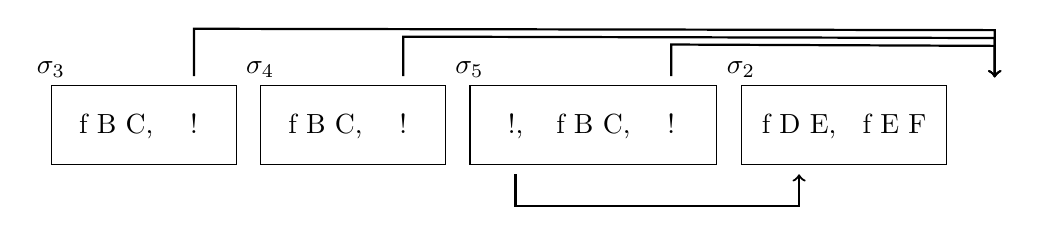
\begin{tikzpicture}[baseline]

\matrix (outer) [matrix of nodes,
                 nodes={draw, minimum width=0.5cm, minimum height=1cm, anchor=center},
                 column sep=0.3cm, row sep=0.3cm] {
\phantom{AAAAAAAA} & \phantom{AAAAAAAA} & \phantom{AAAAAAAAAAA} & \phantom{AAAAAAAAA} &  \node[draw=none] (A) {\phantom{xx}};\\
};

\matrix (inner1) [matrix of nodes,
                 nodes={minimum size=0.6cm},
                 column sep=0.1cm, row sep=0.1cm] at (outer-1-1.center) {
\subnode{ss11}{f B C}, & ! \\
};

\matrix (inner2) [matrix of nodes,
                 nodes={minimum size=0.6cm},
                 column sep=0.1cm, row sep=0.1cm] at (outer-1-2.center) {
\subnode{ss22}{f B C}, & ! \\
};

\matrix (inner3) [matrix of nodes,
                 nodes={minimum size=0.6cm},
                 column sep=0.1cm, row sep=0.1cm] at (outer-1-3.center) {
\subnode{ss33}{!}, & f B C, & ! \\
};

\matrix (inner4) [matrix of nodes,
                 nodes={minimum size=0.6cm},
                 column sep=0.1cm, row sep=0.1cm] at (outer-1-4.center) {
\subnode{ss44}{f D E}, & f E F \\
};


\matrix (innerL) [matrix of nodes,
                 nodes={minimum size=0.6cm},
                 column sep=0.1cm, row sep=0.1cm] at (A.center) {
\phantom{x} \\
};

\draw[->, thick]
  ($(inner1-1-2.north)+(0,0.3)$) -- ++(0,0.6)  
  -- ($(innerL-1-1.north)+(0,0.9)$)            
  -- ($(innerL-1-1.north)+(0,0.3)$);           

\draw[->, thick]
  ($(inner2-1-2.north)+(0,0.3)$) -- ++(0,0.5)  
  -- ($(innerL-1-1.north)+(0,0.8)$)            
  -- ($(innerL-1-1.north)+(0,0.3)$);           

\draw[->, thick]
  ($(inner3-1-3.north)+(0,0.3)$) -- ++(0,0.4)  
  -- ($(innerL-1-1.north)+(0,0.7)$)            
  -- ($(innerL-1-1.north)+(0,0.3)$);           

\draw[->, thick]
  ($(inner3-1-1.south)-(0,0.3)$) -- ++(0,-0.4)  
  -- ($(inner4-1-1.south)-(0,0.7)$)            
  -- ($(inner4-1-1.south)-(0,0.3)$);           

\node at ($(outer-1-1.north west)+(-0,0.2)$) {$\sigma_3$};
\node at ($(outer-1-2.north west)+(-0,0.2)$) {$\sigma_4$};
\node at ($(outer-1-3.north west)+(-0,0.2)$) {$\sigma_5$};
\node at ($(outer-1-4.north west)+(-0,0.2)$) {$\sigma_2$};
\end{tikzpicture}
\end{minipage}



\begin{tikzpicture}[overlay,remember picture]
\draw[->] (ss1) to[in=270, out=270] (ss11);
\draw[->] (ss2) to[in=270, out=270] (ss22);
\draw[->] (ss3) to[in=270, out=270] (ss33);
\draw[->] (ss4) to[in=270, out=270] (ss44);
\end{tikzpicture}

\end{document}